\section{Model2DRigid\-Car\-Forward  Class Reference}
\label{classModel2DRigidCarForward}\index{Model2DRigidCarForward@{Model2DRigid\-Car\-Forward}}
A rigid car-like robot that can only go forward in a 2D world. 


{\tt \#include $<$model2d.h$>$}

Inheritance diagram for Model2DRigid\-Car\-Forward::\begin{figure}[H]
\begin{center}
\leavevmode
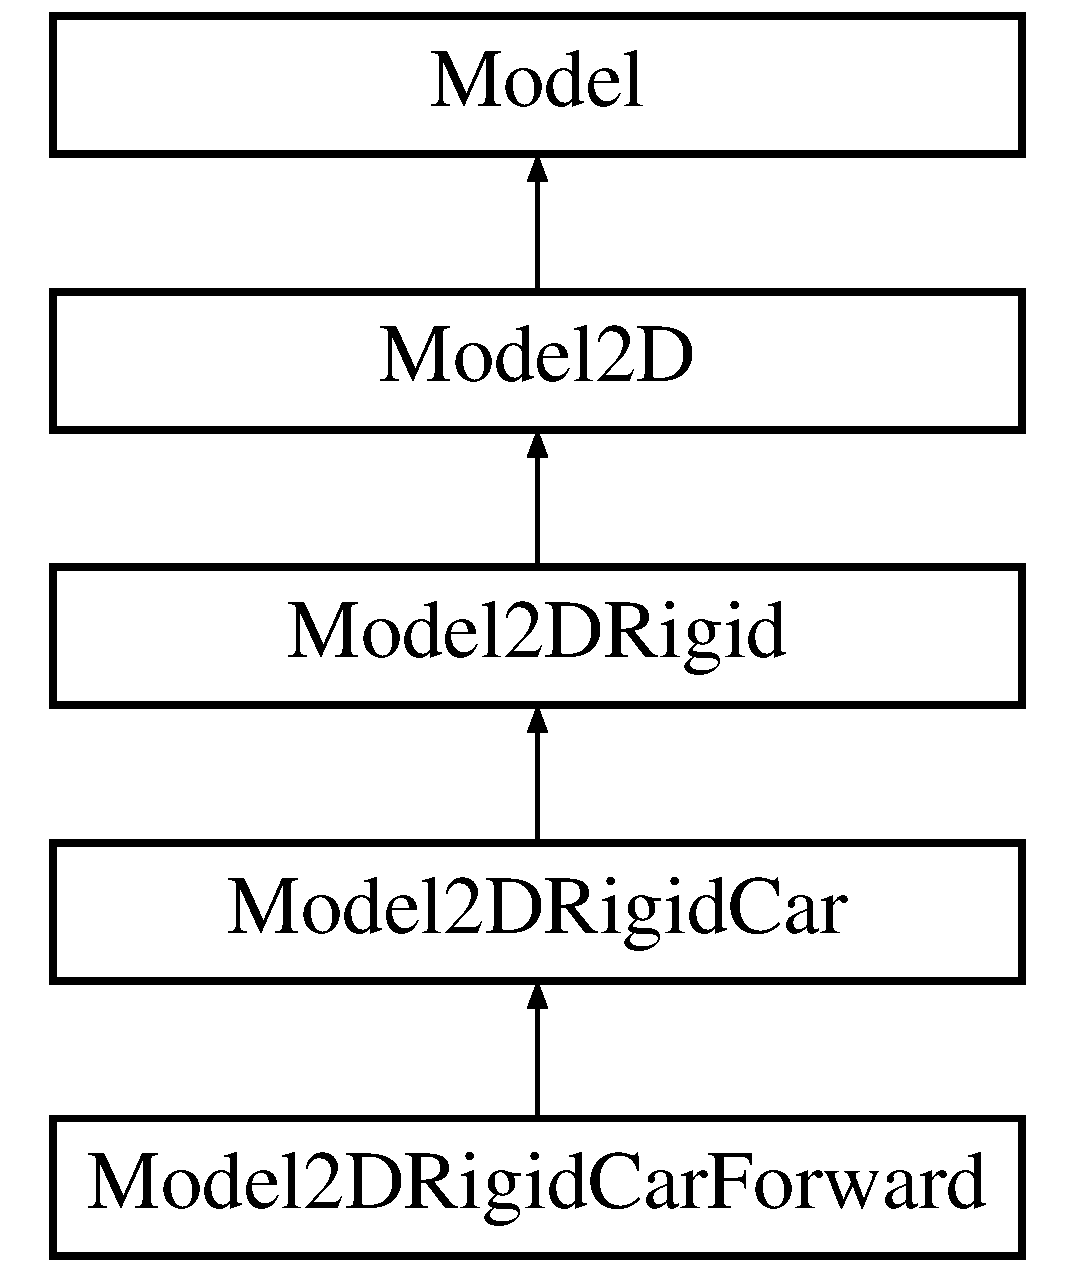
\includegraphics[height=5cm]{classModel2DRigidCarForward}
\end{center}
\end{figure}
\subsection*{Public Methods}
\begin{CompactItemize}
\item 
{\bf Model2DRigid\-Car\-Forward} (string path)
\item 
virtual {\bf $\sim$Model2DRigid\-Car\-Forward} ()
\end{CompactItemize}


\subsection{Detailed Description}
A rigid car-like robot that can only go forward in a 2D world.



\subsection{Constructor \& Destructor Documentation}
\index{Model2DRigidCarForward@{Model2DRigid\-Car\-Forward}!Model2DRigidCarForward@{Model2DRigidCarForward}}
\index{Model2DRigidCarForward@{Model2DRigidCarForward}!Model2DRigidCarForward@{Model2DRigid\-Car\-Forward}}
\subsubsection{\setlength{\rightskip}{0pt plus 5cm}Model2DRigid\-Car\-Forward::Model2DRigid\-Car\-Forward (string {\em path} = \char`\"{}\char`\"{})}\label{classModel2DRigidCarForward_a0}


\index{Model2DRigidCarForward@{Model2DRigid\-Car\-Forward}!~Model2DRigidCarForward@{$\sim$Model2DRigidCarForward}}
\index{~Model2DRigidCarForward@{$\sim$Model2DRigidCarForward}!Model2DRigidCarForward@{Model2DRigid\-Car\-Forward}}
\subsubsection{\setlength{\rightskip}{0pt plus 5cm}Model2DRigid\-Car\-Forward::$\sim$Model2DRigid\-Car\-Forward ()\hspace{0.3cm}{\tt  [inline, virtual]}}\label{classModel2DRigidCarForward_a1}




The documentation for this class was generated from the following files:\begin{CompactItemize}
\item 
{\bf model2d.h}\item 
{\bf model2d.C}\end{CompactItemize}
